\documentclass{sigchi}

% Use this command to override the default ACM copyright statement (e.g. for preprints). 
% Consult the conference website for the camera-ready copyright statement.


%% EXAMPLE BEGIN -- HOW TO OVERRIDE THE DEFAULT COPYRIGHT STRIP -- (July 22, 2013 - Paul Baumann)
% \toappear{Permission to make digital or hard copies of all or part of this work for personal or classroom use is 	granted without fee provided that copies are not made or distributed for profit or commercial advantage and that copies bear this notice and the full citation on the first page. Copyrights for components of this work owned by others than ACM must be honored. Abstracting with credit is permitted. To copy otherwise, or republish, to post on servers or to redistribute to lists, requires prior specific permission and/or a fee. Request permissions from permissions@acm.org. \\
% {\emph{CHI'14}}, April 26--May 1, 2014, Toronto, Canada. \\
% Copyright \copyright~2014 ACM ISBN/14/04...\$15.00. \\
% DOI string from ACM form confirmation}
%% EXAMPLE END -- HOW TO OVERRIDE THE DEFAULT COPYRIGHT STRIP -- (July 22, 2013 - Paul Baumann)


% Arabic page numbers for submission. 
% Remove this line to eliminate page numbers for the camera ready copy
\pagenumbering{arabic}


% Load basic packages
\usepackage{balance}  % to better equalize the last page
\usepackage{graphics} % for EPS, load graphicx instead
\usepackage{times}    % comment if you want LaTeX's default font
\usepackage{url}      % llt: nicely formatted URLs
% llt: Define a global style for URLs, rather that the default one
\makeatletter
\def\url@leostyle{%
  \@ifundefined{selectfont}{\def\UrlFont{\sf}}{\def\UrlFont{\small\bf\ttfamily}}}
\makeatother
\urlstyle{leo}

\usepackage{gensymb}
\usepackage{afterpage}
% see http://tex.stackexchange.com/questions/46055/typesetting-with-inch-symbols-and-sizes-in-inches
% \usepackage{mathpazo}
\usepackage{amsmath}
\def\inch#1{#1''}
\def\ft#1{#1'\thinspace}



% comment macros are in inputmacros.tex
% set up tight list spacing
\usepackage{enumitem} 
\setlist{nolistsep,nosep}

% for toggles
\usepackage{etoolbox}

\newcommand {\studyquote}[1]{\em ``#1''\normalfont}

% CHANGE FROM TOGGLE TRUE TO TOGGLE FALSE FOR NON-ANONYMOUS RENDERING
% http://tex.stackexchange.com/questions/5894/latex-conditional-expression
\newtoggle{anonymous}
%\togglefalse{anonymous}
\toggletrue{anonymous}

% CHANGE FROM TOGGLE TRUE TO TOGGLE FALSE TO HIDE COMMENTS
\newtoggle{comments}
%\toggletrue{comments}
\togglefalse{comments}

% Comment region command (from Wesley Willett)
\usepackage[usenames]{color}
\usepackage[usenames,dvipsnames]{xcolor}
\iftoggle{comments} {
  %if we want to show comments
  \newcommand {\claire}[1]{{\color{Orange}\bf{CT: #1}\normalfont}}
  \newcommand {\sean}[1]{{\color{BlueGreen}\bf{SC: #1}\normalfont}}
  \newcommand {\yang}[1]{{\color{NavyBlue}\bf{YL: #1}\normalfont}}
  \newcommand {\ben}[1]{{\color{violet}\bf{BZ: #1}\normalfont}}
  \newcommand {\bjoern}[1]{{\color{BrickRed}\bf{BH: #1}\normalfont}}
  \newcommand {\achal}[1]{{\color{OliveGreen}\bf{AD: #1}\normalfont}} % can't find another color...
  \newcommand {\changes}[1]{{\color{Red}\bf{#1}\normalfont}}
}{
  %if we don't want to show comments
  \newcommand {\claire}[1]{}
  \newcommand {\sean}[1]{}
  \newcommand {\yang}[1]{}
  \newcommand {\ben}[1]{}
  \newcommand {\bjoern}[1]{}
  \newcommand {\achal}[1]{}
  \newcommand {\changes}[1]{{#1}}
}
\newcommand {\systemname}{HOBS }
\newcommand {\systemnamenospace}{HOBS}

% To make various LaTeX processors do the right thing with page size.
\def\pprw{8.5in}
\def\pprh{11in}
\special{papersize=\pprw,\pprh}
\setlength{\paperwidth}{\pprw}
\setlength{\paperheight}{\pprh}
\setlength{\pdfpagewidth}{\pprw}
\setlength{\pdfpageheight}{\pprh}

% Make sure hyperref comes last of your loaded packages, 
% to give it a fighting chance of not being over-written, 
% since its job is to redefine many LaTeX commands.
\usepackage[pdftex]{hyperref}
\hypersetup{
pdftitle={SIGCHI Conference Proceedings Format},
pdfauthor={LaTeX},
pdfkeywords={SIGCHI, proceedings, archival format},
bookmarksnumbered,
pdfstartview={FitH},
colorlinks,
citecolor=black,
filecolor=black,
linkcolor=black,
urlcolor=black,
breaklinks=true,
}

% create a shortcut to typeset table headings
\newcommand\tabhead[1]{\small\textbf{#1}}


% End of preamble. Here it comes the document.
\begin{document}


% as we discussed last time, the "Sees" and "Line-of-sight" suggests some computer vision direction 
% need a different title for sure, but not in a hurry
\title{Head orientation-based target selection in physical spaces}
%Project GlasSees: Direct Interaction Through Line-of-sight}

\iftoggle{anonymous}{
\author{
 \alignauthor Anonymous for submission\\
    \affaddr{...}\\
    \email{...}\\
  }
}{ %else
  \numberofauthors{1}
  \author{
  \alignauthor Yu-Hsiang Chen$^{\dagger}$, Ben Zhang$^{\dagger}$, Claire Tuna$^{\dagger}$, Yang Li$^{\ddagger}$, Edward Lee$^{\dagger}$, Bj\"orn Hartmann$^{\dagger}$ \\
  \affaddr{$\dagger$: UC Berkeley EECS \& CITRIS Invention Lab \hspace{0.25in} $\ddagger$: Google Research}\\
  \email{sean.yhc@gmail.com, benzh@eecs.berkeley.edu, clairetuna@gmail.com, yangli@acm.org, eal@eecs.berkeley.edu, bjoern@eecs.berkeley.edu}
  }
}

\maketitle

\begin{abstract}
%!TEX root = uist14.tex

%% Yang suggests: Interacting with smart objects in the physical space efficiently is a realistic challenge as these objects become ubiquitous. In this paper, we contribute HOBS, a set of novel methods for selecting physical objects at a distance using infrared-sensed head orientations. We augment a commercial head-worn device, Google Glass, with an infrared (IR) emitter to select targets equipped with IR receivers. We present the iterative design process of our methods, involving a series of interaction technique and hardware design and user evaluations....
Emerging head-worn computing devices can enable interactions with smart objects in physical spaces.
%
We present the iterative design and evaluation of \systemname -- a Head-Orientation Based Selection technique for interacting with these devices at a distance. We augment a commercial wearable device, Google Glass, with an infrared (IR) emitter to select targets equipped with IR receivers. Our first design shows that a naive IR implementation can outperform list selection, but has poor performance when refinement between multiple targets is needed. A second design uses IR intensity measurement at targets to improve refinement. To address the lack of natural mapping of on-screen target lists to spatial target location, our third design infers a spatial data structure of the targets enabling a natural head-motion based disambiguation.
%
Finally, we demonstrate a universal remote control application using HOBS and report qualitative user impressions.

\end{abstract}

\keywords{
  Wearable computing; tangible; smart devices; remote control; glass; infared
}

%% refer to http://www.acm.org/about/class/ccs98-html
\category{H.5.2.}{Information Interfaces and Presentation (e.g. HCI)}{Interaction styles (e.g., commands, menus, forms, direct manipulation)}.

\vfill\eject

%!TEX root = sui14.tex
\vfill
\section{Introduction}
%\bjoern{We should see if we can change language in a few places to strengthen the connection to ``Spatial User Interaction", the title of the conference.}

%% from the swarm vision to the necessity of selection
The number of smart objects in our environment with embedded computation and communication has grown rapidly. These objects are all potential targets for interaction. To initiate {\em spatial interactions}, a user needs to first acquire the target object -- a fundamental task that has been extensively studied in graphical user interfaces, but not yet well-explored in {\em physical spaces}.

\changes{Today, companies like Samsung and Whirlpool are making smart appliances with companion applications that use smartphones as {\em universal remote controls}. With these applications, the user can select a device from a list in order to control it with a device-specific user interface. However, this method faces {\em naming} issues (i.e. ``what do we name the lamp on the left?'') and {\em scaling} issues as the number of controlled devices increases. These solutions also present a necessarily flawed mapping from the positions of the appliances in the rich, 3-dimensional world to their place in a 1D or 2D list presented on the screen. }
%
%% previous approaches are limited
Past research has used direct aiming at target devices in space with phones to overcome these problems~\cite{beigl_point_1999,patel_2-way_2003}. Such techniques have a few drawbacks: the aiming device first has to be retrieved; the user's hands have to be free for operation; and the user's visual attention is split between looking down at a screen and out at targets in the world. 

%% introducing head-worn computing and head orientation
Emerging head-worn computing devices do not require retrieval since the devices are already worn; they may enable hands-free or uni-manual interactions; and they offer near-eye or see-through displays to present information in the wearer's field of view. We thus investigate how such computing devices may be used for the selection and control of devices in physical spaces. Head-worn devices can naturally exploit the user's head orientation, an important (but imprecise) indicator of the user's {\em locus of attention}~\cite{raskin}. It suggests the general direction, but not the particular point of focus. We draw an analogy to assistive area cursors and adapt area cursor techniques~\cite{kabbash1995prince,worden1997making,findlater2010enhanced} for physical selection. Such techniques employ a two-step selection process: a {\em coarse} selection of an area of interest, followed by a {\em refinement} to select a target within that area.

In this paper, we describe the iterative development and evaluation of \systemnamenospace, an area-selection technique that can be readily implemented with small hardware changes to emerging head-worn devices. We augment Google Glass\footnote{\url{http://www.google.com/glass/start/}} to enable infrared (IR) communication between Glass and target appliances. We contribute and evaluate new methods for addressing selection ambiguity in this context. In all our techniques, the emitted IR beam %(a diameter of 30-60cm and distance up to 8m)%
 provides an initial {\em coarse} selection area (illustrated in Figure~\ref{fig:teaser} {\em left}). To {\em refine} selection when multiple targets have received IR signals, we describe and evaluate three techniques:

 Our {\em Naive IR} technique shows an alphabetically ordered disambiguation list on the near-eye display (Figure~\ref{fig:teaser} center). A study with $14$ participants finds that target acquisition with naive IR targeting is preferred by users and is faster than pure list selection without IR, but refinement is still time consuming.

Our {\em Intensity IR} technique improves refinement as target objects compare IR received signal strength (RSS). This value allows the system to eliminate some peripheral targets and to re-order the refinement interface's list by their intensity values. For example, in Figure~\ref{fig:teaser} of {\em Intensity IR} technique, device 5 is eliminated first and the list is re-ordered based on the intensity readings. A second study with $10$ participants shows that {\em Intensity IR} successfully reduces both the probability of needing to do refinement as well as the time spent in list navigation when compared to {\em Naive IR}.

Our final {\em Head-motion Refinement} addresses the lack of a natural mapping when users select a target in the refinement step using their device's touchpad --- the axes of motion do not map directly to the spatial layout of target devices in a room. We first learn the relative spatial structure of the targets using Glass' orientation sensors. Users can then perform head movements to change selections to spatially adjacent targets (see the right of Figure~\ref{fig:teaser}). For example, nodding down to select the target below current selection, or tilting right to select the next target on the right. We present preliminary feedback from participants on this technique.

We also demonstrate an example application of our technique used as a remote control of smart appliances such as lighting and TV sets: a user looks at the appliance he wishes to control and confirms selection by tapping. An appliance-specific user interface is then shown on the user's near-eye display for further interactions. 

%Orientation-based selection enables a wide range of context-aware applications. Examples include smart home remote control, break reminder monitor starer, museum attention tracking, indoor positioning, etc. In Figure\,\ref{fig:teaser}, it's a demonstration of the ``universal remote control'' scenario. The user can easily select the smart appliances by simply looking at it's general direction and confirm such selection with either voice command or by tapping the Glass input pad. Then an appliance-specific control UI will be shown on the head-mounted display. For this application, we have asked 14 participants to try the system and we report the qualitative results from them performing home automation tasks.


% In summary, this paper makes the following contributions:
% \begin{itemize}
% \item We presented our three iteractions of design.
% \item We present evaluations that compare head orientation targeting to list selection and quantify the benefits of automatic disambiguation.
% \item We demonstrate a home appliance remote control application built on top of our selection technique.
% \end{itemize}



%%% Local Variables: 
%%% mode: latex
%%% TeX-master: "sui14"
%%% End: 

%!TEX root = sui14.tex
\section{Background and Related Work}
Our approach is related to head- and eye-controlled interfaces, area cursors and prior work on hardware devices for pointing in physical spaces.

\vfill
\ben{make sure no section title appears at the end of any column.}
\subsection{Head and Gaze Input}
\changes{Head movement has long been used for virtual camera control in VR applications~\cite{pausch_user_1993} and as an assistive input technology for cursor control of desktop applications~\cite{radwin1990method}. However, it is notable that human neck muscles have a lower bandwidth than other muscle groups, e.g., the wrist~\cite{card_morphological_1991}.}
%
%Card, summarizing other work, shows that neck muscles are a poor muscle group for pointing in general: neck muscles only have a bandwidth of about $4.2bits/s$ (compared to $23bits/s$ of wrist muscles used by a standard mouse~\cite{Card:1991:MAD:123078.128726}. 
%
Prior work often focused on head orientation for controlling graphical interfaces; in contrast, we apply this modality to selection in physical spaces.

Gaze can also be used to control graphical user interfaces~\cite{kumar2007eyepoint}. While there are wearable gaze trackers~\cite{bulling2009wearable}, turning information about a concrete point in space where a user is looking into a selection requires a map with known target locations.
Our system works through point-to-point IR communication and does not require an {\em a priori} map or markers. Target objects in the environment can also be equipped with individual cameras that watch the user~\cite{smith2013gaze,vertegaal2005media}. Such an approach can enable similar benefits as our approach, but is computationally more expensive than our single-pixel sensor solution and may not work at greater distances or angles, because it relies on finding the user's pupils in a camera image.

%Our work is closer in spirit to Selker's headworn system~\cite{Selker:2001:EGE:634067.634176}.

\subsection{Area Cursors}
\changes{
In 2D area cursors for GUIs, the activation area of the cursor is enlarged, which facilitates acquiring smaller targets~\cite{kabbash1995prince}. We argue that head orientation pointing has analogous characteristics (limited pointing performance and accuracy). Area cursors are especially appropriate for individuals with motor control impairments or difficulties~\cite{worden1997making,findlater2010enhanced}. Similar ideas have also been extended into 3D to provide selection with progressive refinement in 3D scenes~
\cite{bacim2013design}. In all area and space cursors, the large activation area can lead to multiple targets being selected and disambiguation is needed. This paper describes the trade-offs between several disambiguation approaches.


%We conceptualize area pointing as a two-stage process: in the {\em coarse} phase, which we call {\em scanning}, users move so the activation area intersects with the target object (and possibly other, unintended targets). In the {\em refinement} phase, they adjust so only the intended target will be selected. Many disambiguation techniques are possible for refinement -- this paper describes the trade-offs between several of them.
}

\subsection{Pointing in Physical Spaces}
Rukzio ~\cite{rukzio_experimental_2006} studied alternative methods for selecting devices in physical spaces and found that users strongly preferred either tapping target appliances with a mobile device or pointing at a distance to browsing a list.

Several approaches to spatial selection with handheld devices~\cite{beigl_point_1999,patel_2-way_2003,wilson_xwand:_2003,schmidt_picontrol:_2012,kemp_point-and-click_2008} or finger-worn devices~\cite{merrill_augmenting_2007} exist. 
%and exchanging information with smart infrastructure sensor networks ~\cite{lifton_tricorder:_2007,mittal_ubicorder:_2011,costanza_sensortune:_2010}. 
In some techniques, users select objects of interest with laser pointers. The laser dot provides immediate visual feedback to the user about what is being selected; however, its small target area makes it poorly matched to head orientation input.
Other approaches rely on virtual room models in which a user's location is estimated using IMU-based orientation sensing~\cite{wilson_xwand:_2003,lifton_tricorder:_2007} -- in contrast, our technique does not require a static map ahead of time.
%Other targeting systems use IR with handheld pointers~\cite{swindells_that_2002} as well as wearable devices such as rings and Bluetooth audio earpieces~\cite{merrill_augmenting_2007} to connect to smart devices. 
Our system tackles an unresolved issue of prior approaches -- navigating an area dense with potential targets and resolving selection ambiguity.

\subsection{Vision- and Projection-Based Target Selection}
\changes{Many alternative solutions for detecting devices in contained spaces
rely on computer-vision recognition of printed tags on devices. Unfortunately,
these methods either impose significant constraints on the camera used for
detection~\cite{Bokode}, require large or obtrusive tags~\cite{Dataglyphs}, or
are designed to work specifically at short distances~\cite{CyberCode}. Passive
markers also cannot show visual feedback in the environment.  Handheld
projectors can both display a user interface in space and communicate control
information optically, e.g., by encoding information temporally (using Gray
codes in Picontrol~\cite{schmidt_picontrol:_2012} and RFIG
Lamps~\cite{raskar_rfig_2004}) or spatially (using QR codes in the infrared
spectrum in SideBySide~\cite{willis_sidebyside:_2011}). Our solution is similar
in spirit but requires only small, low-cost IR emitters and detectors.
\bjoern{need a stronger statement here}} \achal{Tried emphasizing the smaller
requirements, not sure what else we can say.}

%However, visible tags at appropriate sizes may be rejected by users because of their negative aesthetic effect on the space.

%\subsection{Markers and Vision Methods}
%\achal{Not sure where to put this, feel free to move.}
%
%\ben{For CV, I think related work is one option to go; however, the requirement of being related work is that -- we need to reference them. There are a few examples ``require large, obtrusive tags, and inevitably lack feedback from passive devices in the environment'' which should be referenced. That's why I am thinking of putting this to discussion.}
%


%\ben{Reviewers suggest considering computer vision-based techniques with markers in the environment (such as %QR codes, or Bokode [Mohan] which extends the working distance to a few meters for visual tags). We considered this direction and found several drawbacks, including computational complexity, low accuracy when targets are far, the absence of real-time environment feedback with passive tags, and aesthetic issues with QR codes. While we don't claim our choice of IR is optimal, it has important advantages -- it is low-cost, readily available and quite suitable for area selection. We can weaken our claim and add explanations of how disambiguation techniques might generalize to other methods of implementing target identification.}

%\achal{Read and discussed the Bokode paper and CV in general. Unsure about what
%to do regarding "weakening our claim."}


%\ben{new related works from reviewers}. \bjoern{folded in}
%\changes{RFIG Lamps and photosensing wireless tags [Raskar et al] use a projector and data is encoded in each pixel so that tags can localize themselves for target selection. Our IR emitter, a relatively low-cost solution, doesn’t have this feature but shares the commonality of covering an area for the ease of selection. At the end of their paper, they envision an IR-based system to solve ambient light problems. Our work lies in that direction and also contributes evaluations with user studies.
%Progressive Refinement [Bacima] studies several progressive refinement selection modalities, which is close to our two-stage selection; but our contexts are head-orientation as it reflects users' point of interest.
%}

%
\section{Background}
\label{sec:background}


%% Bjoern: I would mostly rely on prior literature here. There are neck-controlled joysticks for users with disabilities that are probably useful to look at. see below.
 
%% YL: I also think we should briefly cover how people used to detect head-orientatation. I don't have references at hand and the only paper I can recall is Michel's paper. I think Pourang Irani has papers in this area too. Overall I think previous ways are too heavyweight. In comparison, your way of acquiring head orientation is more effective and lightweight.

In this section, we will first provide some background about human's neck muscle kinectics. Given that constrain, we think the right way to achieve head-orientation based targeting should be using the area selection technique. This motivates our selection of using IR to capture users' head orientation and also the carefully design of the disambiguation technique.



%%% Local Variables: 
%%% mode: latex
%%% TeX-master: "uist14"
%%% End: 

%!TEX root = uist14.tex


\bjoern{The design and prototyping sections are very thorough, but too long. If we want to submit a shorter paper we need a more concise description. We generally don't need to describe the sequence of steps we took to prototype something, just the final solution and the motivation for each decision. If I wanted to describe the whole system on one page, i'd probably structure it as follows:}
\section{Interaction technique description}
One paragraph about how the technique works from the user's perspective.
\section{Implementation: IR-based Head-Orientation}
\subsection{Head-worn emitter}
Our selection technique adds an IR emitter to a wearable device frame in line with the wearer's saggital (font-to-back) plane (see Figure). IR is a suitable technology because it is directional. The angle of emittance leads to a cone-shaped area coverage. Many different emitter angles are commercially manufactured; we use $x^circ$, which yields a selection area of diameter Y at distance Z (part number XXXX).
We attach the IR emitter to the frame with a repositionable 3D-printed mount that can account for individual differences in head shape (users adjust the mount so the emitter points directly forward, level to the ground.)

\subsection{Target receivers}
Each selectable target is equipped with IR receivers. We are interested in sensing two things: 1) IR communication and 2) IR intensity. Common IR receivers have automatic gain control built in and hide received signal strength. We therefore add an IR intensity sensor. In a commercial application, a single sensor that both decodes and reports RSSI could be designed.
\subsubsection{Visual feedback}
...
\subsection{Wireless communication}
(describe that we only use IR initially, then jump to RF-based communication.)

\section{System Design and Prototyping}
\label{sec:syst-design-prot}

This section describes the design and implementation of our prototype system. We start by summarizing the design considerations in this head-orientation targeting, and for each consideration, we make the choice of commercial off-the-shelf (COTS) components. Afterwards, we conclude this section by a depiction of the overall system architecture that is used for both our study and future application development. 

\subsection{Design Considerations}
\label{sec:design-cons}

To effectively enables the physical targeting based on user's head movement, and build such a platform for applications, we have come up with the following design considerations and the justification for each.

{\bf Directional area selection:} To be aligned with the user's head orientation, the sensing modality should be directional. Merely direction is not enough, from Section~\ref{sec:background}, the head muscle's fundamental limitation and Fitts' law imposes us to choose an area selection technique. However,  with a larger coverage area, there will be a higher chance for disambiguation. We should find the proper technique that achieves area selection while still providing ways for a more fine-grained resolution.

% the two visual feedback seems a bit random...
{\bf Leverage visual feedback:} Since the user cannot see his own head orientation, there should be some effective ways to provide feedback to the users. We consider two types of visual feedbacks. The first comes from the environment which enables instantaneous visual cue while the user is looking around. The second should remain unchanged even if the users' head orientation has changed; in such a way, further interactions are enabled without imposing the burden of staring. But such a display shouldn't distract the user's current line-of-sight attention -- which means a near-eye display is better than using a hand-held device. 

% A calmer~\cite{weiser_coming_1997} approach is to locate visual feedback about selection targets in the environment, to prevent distraction and interruption. Such feedback should be delivered instantaneously, while users look around a room.

{\bf Flexible communication:} The system is for the interaction with the environment, therefore the communication among devices should be flexible. Especially there would be a consensus problem if the end-nodes are not agreeing on what the user is looking at. The communication would be necessary for resolving the inconsistency in such a distributed environment. Also providing a flexible communication capability can make the system as a platform for other applications. 

{\bf Adjustable angle:} From our pilot study, we have learned that human's head orientation pointing is biased for each person. In order to align area selection technique, there should be ways to adjust or calibrate the covered area.

These design considerations find their expression in our selection of techniques in the following few subsections.

\subsection{IR as beam cursor}
\label{sec:ir-as-beam}

For the directional area selection technique, we have chosen to use infrared (IR) for a couple of reasons.  

First, the signal characteristics of IR makes it suitable for directional area selection. There are a wide range of viewing angles that we can choose (DigiKey offers IR emitters from $4^\circ$ to $240^\circ$, however, most are around $20^\circ$ of viewing angle). This leads to a cone shape-like area coverage and can be well-aligned with human's line of sight. 

Second, for the disambiguation consideration, since the infrared illuminance falls off with respect to both the offset angle from the center and the distance to the emitter, even though the signal might cover multiple targets, using the intensity from the receivers can help disambiguation.  
% for the 4 degree to 240 degree, I used information from http://www.digikey.com/product-search/en/optoelectronics/infrared-uv-visible-emitters/524328?k=IR

In addition, IR has been used for remote control for many years. The emitters and receivers are fairly cheap to manufacture; and it's easy for integration with existing devices. 
What's more, IR is immune to most interference sources. The ambient IR might influence the IR receivers' intensity reading, however with simple IR signal validation, the receiver is still safe. There might be issues for signal reflection, either bouncing from the ground to the target or bouncing back to the opposite direction. However, such visual feedback is not aligned with the user's attention so no further action from the user might be taken; or the genuine target could easily beat the false positive since the one with reflection tends to travel a longer distance, making the signal strength smaller.

Therefore, we can attach an IR emitter to capture the head orientation and install some IR receivers in the environment for both signals detection and intensity reading. For our prototype, we have found some COTS components for IR. 
The IR emitter is the one from OSRAM Opto Semiconductors Inc with manufacturer part number SFH 4545. From the data-sheet, it has a view angle of $10^\circ$. Part of the reason we have chosen it is because the radiant intensity can quite high if we provide it with sufficient current flow (550mW/sr @ 100mA). We can then easily adjust it using a resistor to satisfy different demands. 
% transmitter webpage: http://www.digikey.com/product-search/en?x=0&y=0&lang=en&site=us&KeyWords=475-2919-ND
For the IR receiver, we use 38.0kHz IR Receiver Modules from Vishay Semiconductor Opto Division (manufacturer part number TSOP38238). 
% receiver webpage http://www.digikey.com/product-detail/en/TSOP38238/751-1227-ND/1681362
In order to read the IR intensity, we integrates another IR light-to-voltage converter from AMS-TAOS USA Inc (manufacturer part number TSL267-LF) which is pretty sensitive to IR irradiance. 
% http://www.digikey.com/product-detail/en/TSL267-LF/TSL267-LF-ND/3095052

We use Arduino platform for the prototyping, and there is an easy-to-use IR library\footnote{\url{https://github.com/shirriff/Arduino-IRremote}} where we can customize the IR signal for both transmission and reception. To read the IR intensity, an 10-bit ADC is attached to the output of TSL267-LF which gives a reading from 0 to 1023. 

\subsection{Environment LEDs and Head-up display}
\label{sec:head-up-display}
As we have argued for the visual feedback design considerations, the environment should provide instantaneous visual cue to respond to user's head orientation. This can be easily achieved with 1-bit LEDs on each devices that has an IR receiver. For the visual feedback that is persistent even when the user's head orientation has changed, we have considered a few COTS solutions that support the head-up display, and ended up with Google Glass because it's easy to program (it supports standard Android programming) and the device is also light-weight for everyday use. At the time of writing, we have Google Glass running Android 4.0.4 (software version: XE12). 

\subsection{Wireless Communication}
\label{sec:wirel-comm}

There are many choices of wireless communication techniques that we could consider to accompany IR's directional targeting. WiFi, Bluetooth Low Energy (BLE) and 802.15.4 (ZigBee) radio are all candidates for such communications. A detailed comparison is out of the scope of this paper. For our prototype, we have chosen to use XBee ZB\footnote{XBee: http://www.digi.com/xbee/}(based on ZigBee protocol and 802.15.4 radio) for the mesh network because of the ease to program and integration to Arduino platform. The COTS adapter provides an easy-to-use interface where we could use either hardware serial pins or the software serial library to send and receive messages. 

As we mentioned that the communication capability has to be included to resolve the consensus view of head orientation, we use the star topology -- the node which controls IR emission acts as the PAN coordinator. It collects the IR received signal strength (RSS) from each targets and runs a local algorithm to determine which one is the current target. 

Using such an architecture for communication also makes the integration with Google Glass easier. For now, Google Glass is only capable of WiFi and Bluetooth; so we have to add a Bluetooth modem to establish connections with Google Glass\footnote{This is a compromise now, and we are planning to migrate the entire system to BLE once Google upgrade the Glass software to Android 4.4+. The prototype now suffice our demand to run the head orientation study.}. We use BlueSMiRF Silver (WRL-12577) for our prototype. 

\subsection{3D Printed Adjustable Holder}
\label{sec:3d-print-adjust}
To compensate for the bias of each person's line of sight with the IR emitter, we have designed the holder that can be easily attached onto Google Glass while we can adjust the beam angle flexibly.

\begin{figure}[t]
\centering
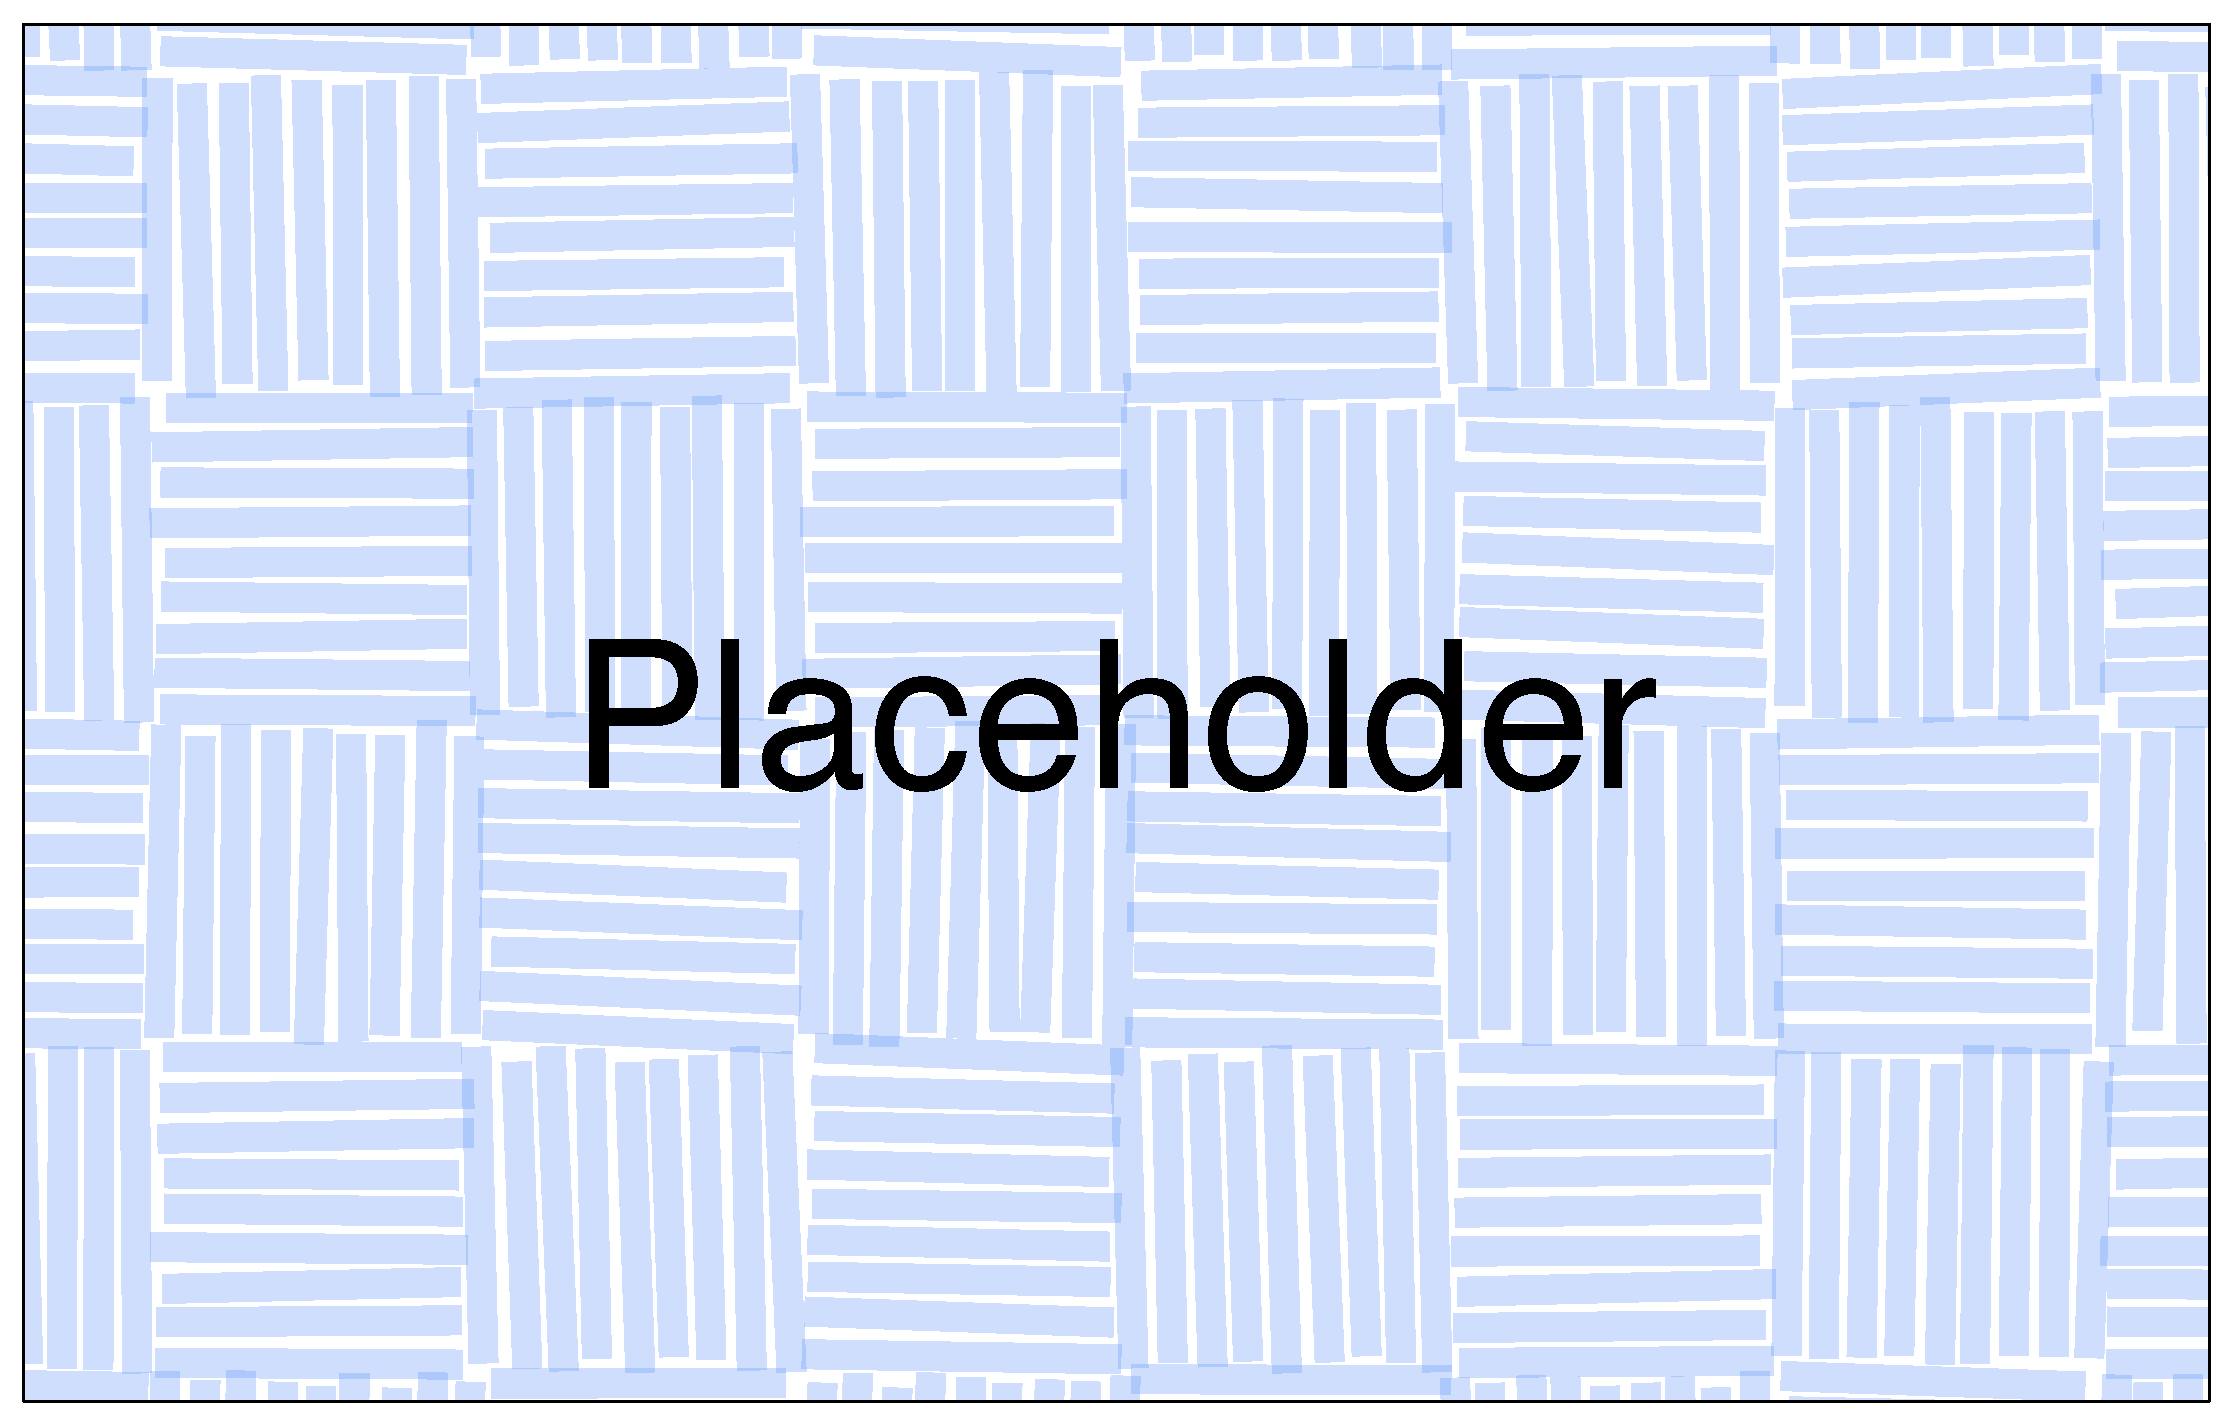
\includegraphics[width=0.9\columnwidth]{figures/placeholder.pdf}
\caption{we should replace this place-holder with Claire's design and printed version.}
\label{fig:3d-holder}
\end{figure}

\subsection{Overall System}
\label{sec:overall-system}
So far we have been discussing separate components that fit our design considerations. To stitch them into a single system, we use the following architecture shown in Figure~\ref{fig:architecture}.

\begin{figure}[t]
\centering
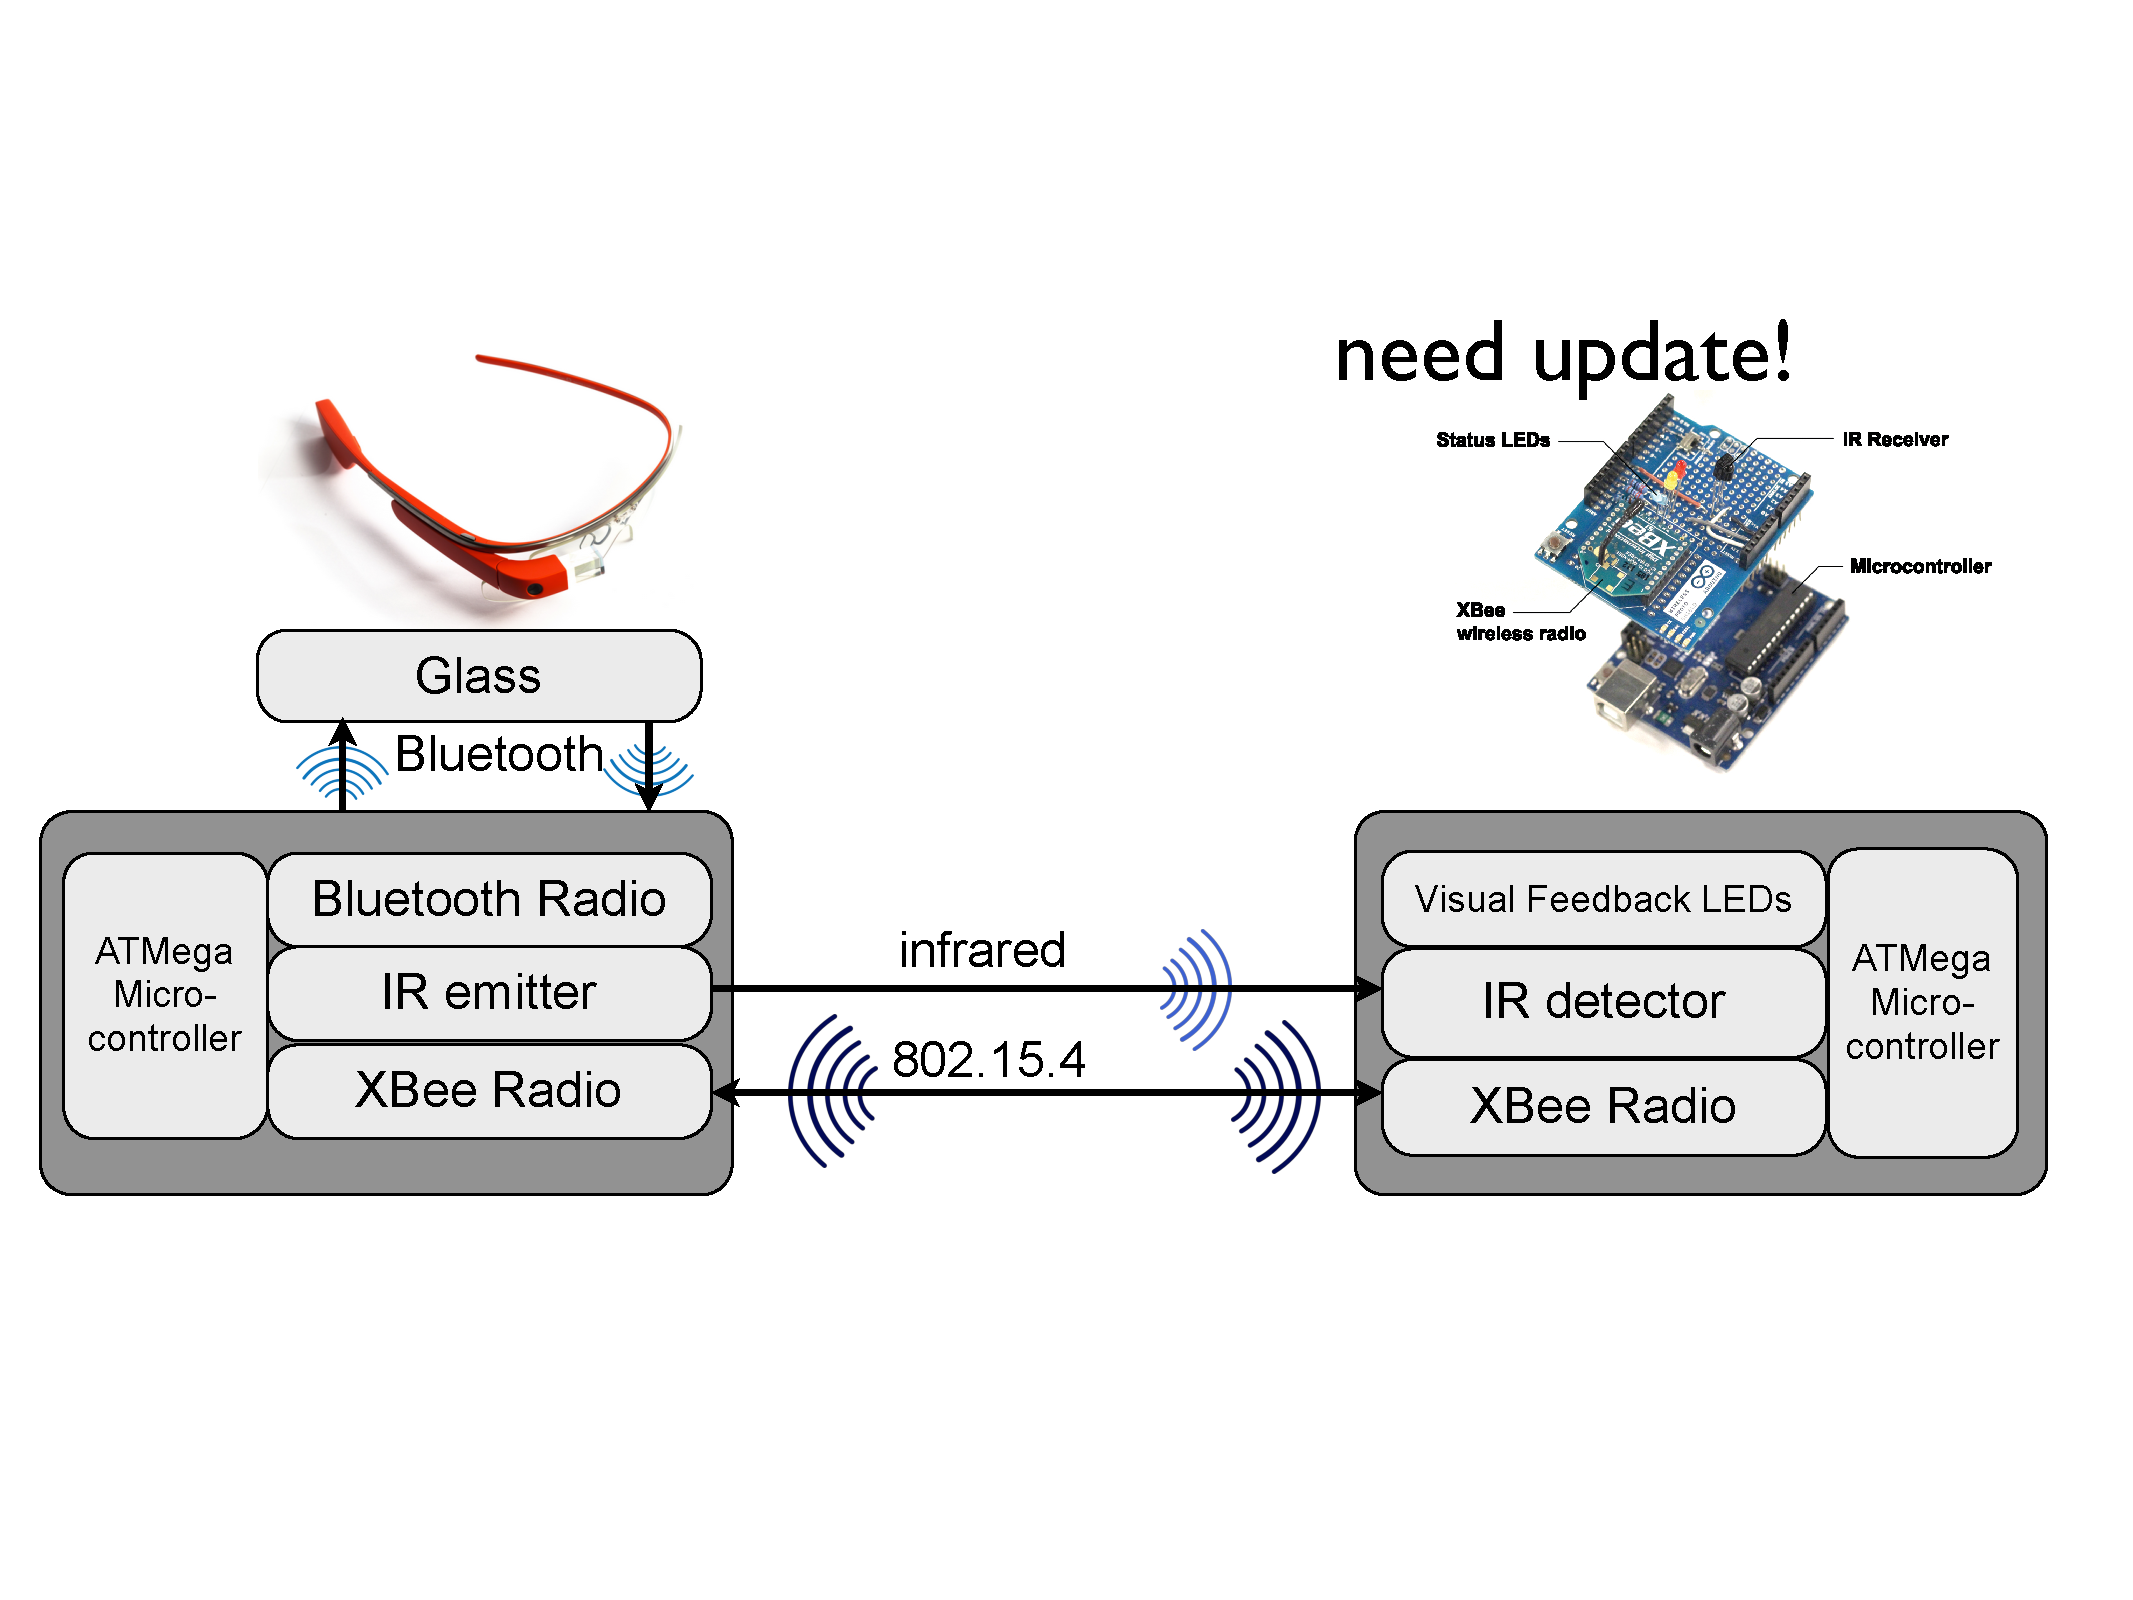
\includegraphics[width=0.9\columnwidth]{figures/architecture.pdf}
\caption{In our system architecture, targeting is captured by IR signal but the confirmation and coordination is over 802.15.4. Google Glass communicates with the system through Bluetooth.}
\label{fig:architecture}
\end{figure}

\ben{this paragraph needs refinement. Maybe a good idea is to use one single sentence to summarize the disambiguation and say we will talk about it in the next section.}
In our system, the microcontroller at the Google Glass side (we will call it the master) takes charge of bridging the end nodes and the Glass. It constantly transmits IR signal no specific connection with any node has been established. When the node receives such signal, they validate the packet and send back IR intensity readings. The master may simply use the IR intensity changes to determine which is the intended targets, or pass the information to Google Glasss where the Glass combines both motion sensor readings with the IR signal intensity to disambiguate. We will leave the algorithm description in the next section. Once a decision has been made, such information will be sent back to the node and the visual feedback is provided to the user. The user is free to adjust during the targeting process, our algorithm will dynamically adjust to the user's head movement. Once the user confirms the targeting, he could easily tap the touchpad. Single tap only enables highlighting, targeting confirmation is done with a second tap. This is the last resort for the user to adjust targets. Since the disambiguation matters to the overall performance, we will focus on the discussion in the next section.

%%% Local Variables: 
%%% mode: latex
%%% TeX-master: "uist14"
%%% End: 

\section{Disambiguation Techniques}
\label{sec:disamb-techn}

This section discusses the three different disambiguation techniques we have proposed.

\subsection{Using IR Intensity}
\label{sec:using-ir-intensity}

\subsection{Using Glass Sensors}
\label{sec:using-glass-sensors}

\subsection{Manual Disambiguation}
\label{sec:manu-disamb}



%%% Local Variables: 
%%% mode: latex
%%% TeX-master: "uist14"
%%% End: 


\section{Evaluation}
\label{sec:evaluation}

This section we present our work on the evaluation and user study.


%%% Local Variables: 
%%% mode: latex
%%% TeX-master: "uist14"
%%% End: 

\section{Applications}
\label{sec:applications}

In this section we describe four possible applications that can be built on top of the head orientation-based selection. We focus our discussion on the ``universal remote control'' system. 

%%% Local Variables: 
%%% mode: latex
%%% TeX-master: "uist14"
%%% End: 


\section{Discussion}
\label{sec:discussion}

We discuss a few issues with the system.
%%% Local Variables: 
%%% mode: latex
%%% TeX-master: "uist14"
%%% End: 

\section{Conclusion}
We introduced a novel method for selecting and controlling smart appliances in physical spaces through  infrared targeting based on head orientation. The design takes advantage of the fact that visual attention can express intention, makes it ituitive and helps users remain their focus in the physical world. It addresses the naming and scaling challenges faced by handheld mobile devices. While we present a prototype approach that requires that the user carry additional hardware, all parts can readily be miniaturized and integrated into future head-worn hardware. We also introduced a disambiguation technique in case head orientation is not sufficient to determine a unique target. We characterized our devices performance, arguing that it is matched well to the amount of head movement people can control without strain. A target acquisition study showed that the technique is efficient; a home control scenario showed promise but also limitations when trying to control complex appliances. As our environment continues to be populated by a swarm of sensing and actuation devices, methods to interrogate and control our smart environments may become increasingly important.
%\section{Acknowledgments}
%We thank our user study participants and the a

\iftoggle{anonymous}{
% no acks in anonymous submission
}{
  \section{Acknowledgments}
  
  This work was supported in part by the TerraSwarm Research Center, one of six centers supported by the STARnet phase of the Focus Center Research Program (FCRP) a Semiconductor Research Corporation program sponsored by MARCO and DARPA. Additional support was provided by a Sloan Foundation Fellowship and a Google Research Award.
}
%figure template:
%\begin{figure}[!h]
%\centering
%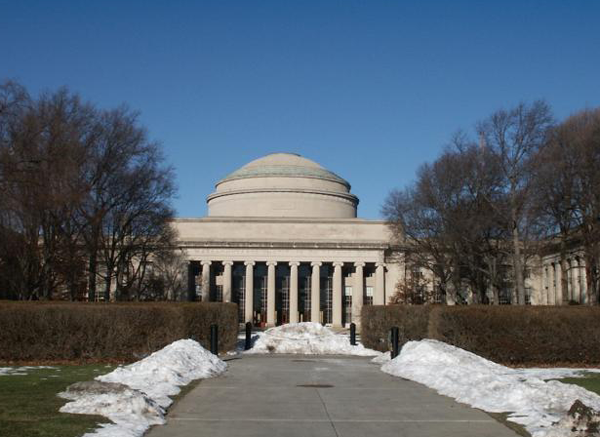
\includegraphics[width=1.0\columnwidth]{Figure1}
%\caption{With Caption Below, be sure to have a good resolution image
%  (see item D within the preparation instructions).}
%\label{fig:figure1}
%\end{figure}

% Balancing columns in a ref list is a bit of a pain because you
% either use a hack like flushend or balance, or manually insert
% a column break.  http://www.tex.ac.uk/cgi-bin/texfaq2html?label=balance
% multicols doesn't work because we're already in two-column mode,
% and flushend isn't awesome, so I choose balance.  See this
% for more info: http://cs.brown.edu/system/software/latex/doc/balance.pdf
%
% Note that in a perfect world balance wants to be in the first
% column of the last page.
%
% If balance doesn't work for you, you can remove that and
% hard-code a column break into the bbl file right before you
% submit:
%
% http://stackoverflow.com/questions/2149854/how-to-manually-equalize-columns-
% in-an-ieee-paper-if-using-bibtex
%
% Or, just remove \balance and give up on balancing the last page.
%
%% \balance

\bibliographystyle{acm-sigchi}
\bibliography{uist14}
\end{document}
